%%%%%%%%%%%%%%%%%%%%%%%%%%%%%%%%%%%%%%%%%
% Beamer Presentation
% LaTeX Template
% Version 1.0 (10/11/12)
%
% This template has been downloaded from:
% http://www.LaTeXTemplates.com
%
% License:
% CC BY-NC-SA 3.0 (http://creativecommons.org/licenses/by-nc-sa/3.0/)
%
%%%%%%%%%%%%%%%%%%%%%%%%%%%%%%%%%%%%%%%%%

%----------------------------------------------------------------------------------------
%	PACKAGES AND THEMES
%----------------------------------------------------------------------------------------
\documentclass{beamer}

\mode<presentation> {

% The Beamer class comes with a number of default slide themes
% which change the colors and layouts of slides. Below this is a list
% of all the themes, uncomment each in turn to see what they look like.

%\usetheme{default}
%\usetheme{AnnArbor}
%\usetheme{Antibes}
%\usetheme{Bergen}
\usetheme{Berkeley}
%\usetheme{Berlin}
%\usetheme{Boadilla}
%\usetheme{CambridgeUS}
%\usetheme{Copenhagen}
%\usetheme{Darmstadt}
%\usetheme{Dresden}
%\usetheme{Frankfurt}
%\usetheme{Goettingen}
%\usetheme{Hannover}
%\usetheme{Ilmenau}
%\usetheme{JuanLesPins}
%\usetheme{Luebeck}
%\usetheme{Madrid}
%\usetheme{Malmoe}
%\usetheme{Marburg}
%\usetheme{Montpellier}
%\usetheme{PaloAlto}
%\usetheme{Pittsburgh}
%\usetheme{Rochester}
%\usetheme{Singapore}
%\usetheme{Szeged}
%\usetheme{Warsaw}

% As well as themes, the Beamer class has a number of color themes
% for any slide theme. Uncomment each of these in turn to see how it
% changes the colors of your current slide theme.

%\usecolortheme{albatross}
%\usecolortheme{beaver}
%\usecolortheme{beetle}
%\usecolortheme{crane}
%\usecolortheme{dolphin}
%\usecolortheme{dove}
%\usecolortheme{fly}
%\usecolortheme{lily}
%\usecolortheme{orchid}
%\usecolortheme{rose}
%\usecolortheme{seagull}
%\usecolortheme{seahorse}
%\usecolortheme{whale}
%\usecolortheme{wolverine}

%\setbeamertemplate{footline} % To remove the footer line in all slides uncomment this line
%\setbeamertemplate{footline}[page number] % To replace the footer line in all slides with a simple slide count uncomment this line

%\setbeamertemplate{navigation symbols}{} % To remove the navigation symbols from the bottom of all slides uncomment this line
}

\usepackage{graphicx} % Allows including images
\graphicspath{{imgGit/}}
\usepackage{hyperref}
\usepackage{booktabs} % Allows the use of \toprule, \midrule and \bottomrule in tables

%----------------------------------------------------------------------------------------
%	TITLE PAGE
%----------------------------------------------------------------------------------------

\title[Initiation GitHub]{Initiation \`{a} GitHub} % The short title appears at the bottom of every slide, the full title is only on the title page

\author{} % Your name
\institute[Universit\'{e} de Rouen] % Your institution as it will appear on the bottom of every slide, may be shorthand to save space
{
Universit\'{e} de Rouen \\ % Your institution for the title page
\medskip
\textit{} % Your email address
}
\date{\today} % Date, can be changed to a custom date

\begin{document}

\begin{frame}
\titlepage % Print the title page as the first slide
\end{frame}

\begin{frame}
\frametitle{vue d'ensemble} % Table of contents slide, comment this block out to remove it
\tableofcontents % Throughout your presentation, if you choose to use \section{} and \subsection{} commands, these will automatically be printed on this slide as an overview of your presentation
\end{frame}

%----------------------------------------------------------------------------------------
%	PRESENTATION SLIDES
%----------------------------------------------------------------------------------------

%------------------------------------------------
\section{Cr\'eation} % Sections can be created in order to organize your presentation into discrete blocks, all sections and subsections are automatically printed in the table of contents as an overview of the talk
%------------------------------------------------

\subsection{Cr\'eation du compte GitHub} % A subsection can be created just before a set of slides with a common theme to further break down your presentation into chunks
\begin{frame}
\frametitle{Cr\'eation du compte GitHub}
\begin{itemize}
\item Afin de proc\'{e}der \`{a} la cr\'{e}ation de votre compte GitHub
\item Rendez-vous sur le site: \href{https://github.com/}{https://github.com/}
\end{itemize}
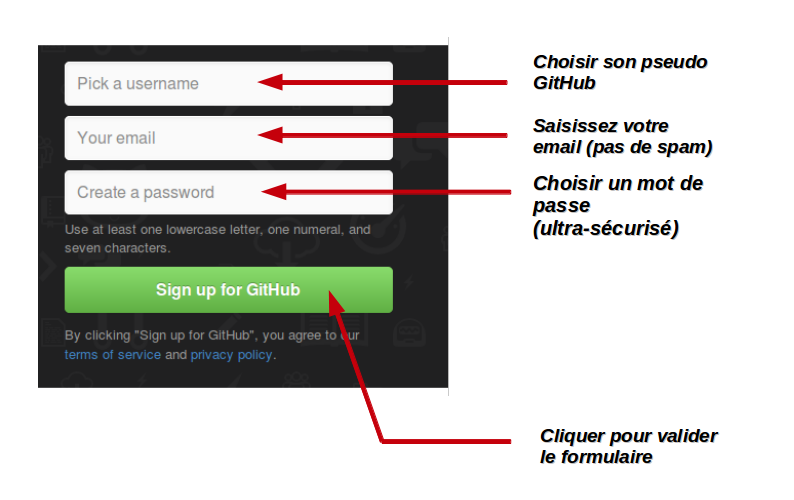
\includegraphics[scale=0.3]{git_hub_home1.png}
\end{frame}

%------------------------------------------------

\begin{frame}
\frametitle{Cr\'eation du compte GitHub}
\begin{itemize}
\item Il s'agit d\'{e}sormais de d\'{e}finir les options comme ci-dessous:
\end{itemize}
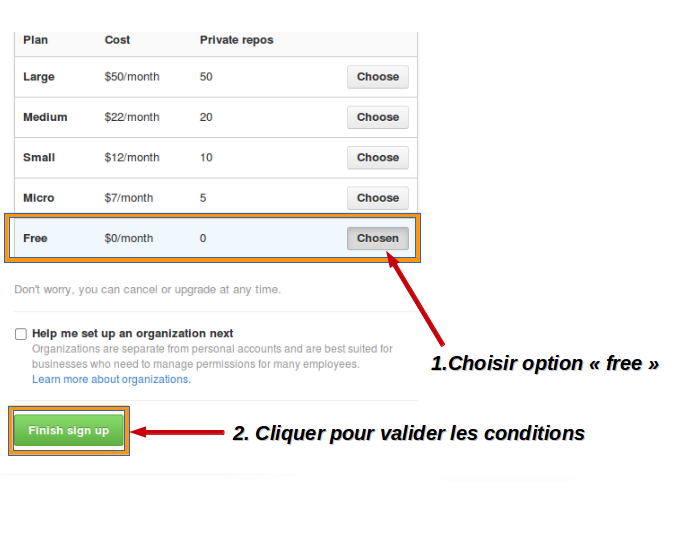
\includegraphics[scale=0.3]{GitHubfininsc.png}
\end{frame}

%------------------------------------------------

\begin{frame}
\frametitle{Cr\'eation du compte GitHub}
\begin{block}{Cr\'eation du compte GitHub fini}
Vous \^{e}tes redirigez vers votre page d'acceuil GitHub.
\end{block}
\end{frame}

%------------------------------------------------



%------------------------------------------------



%------------------------------------------------
\section{Installation}
\begin{frame}
\frametitle{Installation}
\begin{block}{Installation Git}
Pour installer Git, vous avez besoin des biblioth\`{e}ques suivantes: curl, zlib, openssl, expat, libiconv.\\ Par exemple, si vous avez un syst\`{e}me d'exploitation qui utilise yum (tel que Fedora) ou apt-get (tel qu'un syst`{e}me bas\'{e} sur Debian), vous pouvez utiliser l'une des commandes suivantes pour installer les d\'{e}pendances :
\begin{itemize}
\item install curl-devel expat-devel gettext-devel 
  openssl-devel zlib-devel

\item apt-get install libcurl4-gnutls-dev libexpat1-dev gettext 
  libz-dev libssl-dev
\end{itemize}
\end{block}
\end{frame}

%------------------------------------------------

\subsection{Installation sur Windows}\label{Installation sur Windows}
\begin{frame}
\frametitle{Installation}
\begin{block}{Installation Git sur Windows}
\begin{itemize}
\item Rendez-vous sur le site: \href{http://git-scm.com/download/win}{http://git-scm.com/download/win}
\end{itemize}
\end{block}
\end{frame}

%------------------------------------------------

\subsection{Installation sur Linux}\label{Installation sur Linux}
\begin{frame}
\frametitle{Installation}
\begin{block}{Installation Git sur Linux}
\begin{itemize}
\item Debian/Ubuntu \\ \$ apt-get install git
\end{itemize}
\begin{itemize}
\item Fedora  \\ \$ yum install git
\end{itemize}
\begin{itemize}
\item Arch Linux  \\ \$ pacman -S git
\end{itemize}
\begin{itemize}
\item FreeBSD \\ \$ cd /usr/ports/devel/git\\ \$ make install
\end{itemize}

\end{block}
\end{frame}

%------------------------------------------------

\subsection{Installation sur Mac}\label{Installation sur Mac}
\begin{frame}
\frametitle{Installation}
\begin{block}{Installation Git sur Mac}
\begin{itemize}
\item Rendez-vous sur le site: \href{http://git-scm.com/download/mac}{http://git-scm.com/download/mac}
\end{itemize}
\end{block}
\end{frame}


%------------------------------------------------
\section{Utilisation}
\begin{frame}
\frametitle{Utilisation}
\begin{block}{Utilisation Git}
Nous allons voir dans cette section le param\'{e}trage pour la premi\`{e}re utilisation de Git, puis quelques notions pour se d\'{e}placer dans l'arbre et ainsi r\'{e}cup\'{e}rer les mises \`{a} jour.
\end{block}
\end{frame}

%------------------------------------------------

\subsection{Premi\`{e}re utilisation}
\begin{frame}
\frametitle{Utilisation (Premi\`{e}re utilisation)}
\begin{block}{Premi\`{e}re utilisation}
Une fois Git install\'{e}, il faut r\'{e}gler votre identit\'{e} et votre \'{e}diteur de texte si vous le souhaitez.
\end{block}

\begin{block}{Identit\'{e}}
\$ git config \--\--global user.name "YOUR\_USERNAME"\\
\$ git config \--\--global user.email YOUR\_EMAIL
\end{block}

\begin{block}{\'{E}diteur de texte}
\$ git config \--\--global core.editor vim
\end{block}
\end{frame}

%------------------------------------------------
\subsection{Clonage}
\begin{frame}
\frametitle{Utilisation (Clonage)}
\begin{block}{Clonage}
L'objectif est de r\'{e}cup\'{e}rer l'int\'{e}gralit\'{e} du d\'{e}pot de sorte \`{a} cloner le d\'{e}pot distant en local.
\end{block}

\begin{block}{R\'{e}cup\'{e}ration de l'URL du d\'{e}pot}
\'{E}tape 1 : Allez sur votre page d'acceuil Github:  \href{https://github.com/}{https://github.com/}
\end{block}
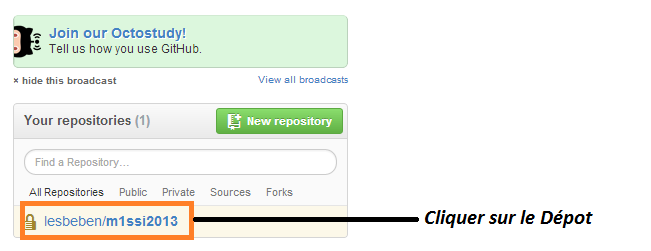
\includegraphics[scale=0.6]{githubhomedepot.png}
\end{frame}

%------------------------------------------------

\begin{frame}
\frametitle{Utilisation (Clonage)}
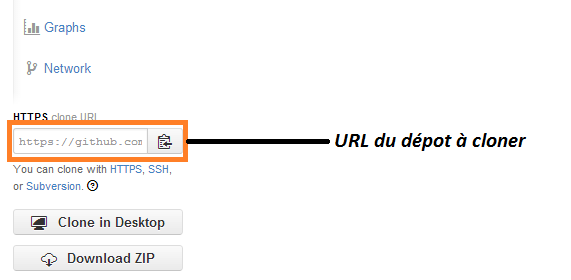
\includegraphics[scale=0.6]{URLdepot.png}
\end{frame}

%------------------------------------------------

\begin{frame}
\frametitle{Utilisation (Clonage)}
\begin{block}{Clonage}
A l'aide du terminal, d\'{e}placez vous dans le r\'{e}pertoire ou vous souhaitez cloner le d\'{e}pot distant puis cloner le r\'{e}pertoire \`{a} l'aide de la commande suivante:\\
\$ git clone [URL]
\end{block}
\end{frame}

%------------------------------------------------

\subsection{D\'{e}placement dans l'arbre}
\begin{frame}
\frametitle{D\'{e}placement dans l'arbre}
\begin{block}{Se d\'{e}placer}
Le git se pr\'{e}sente sous forme d'un arbre dans lequel on peut se d\'{e}placer afin d'en explorer ses branches.
\begin{itemize}
\item \textbf{Lister les branches:} \\
\$ git branch
\item Cr\'{e}er une nouvelle branche: \\
\$ git branch nom-branche
\item \textbf{Changer de branche:} \\
\$ git checkout nom-branche
\end{itemize}
\end{block}
\end{frame}

%------------------------------------------------

\subsection{R\'{e}cup\'{e}ration des mises \`{a} jour}
\begin{frame}
\frametitle{R\'{e}cup\'{e}ration des mises \`{a} jour}
\begin{block}{R\'{e}cup\'{e}ration par fusion du d\'{e}pot distant}
\begin{itemize}
\item \textbf{Mettre \`{a} jour la branche locale en fusionnant la branche distante:} \\
\$ git pull
\end{itemize}
\end{block}
\end{frame}

%------------------------------------------------




%----------------------------------------------------------------------------------------

\end{document} 
